
% !TEX TS-program = pdflatex
% !TEX encoding = UTF-8 Unicode
 
\documentclass[12pt]{report} % use larger type; default would be 10pt
 
\usepackage[utf8]{inputenc} % set input encoding (not needed with XeLaTeX)
 
%%% Examples of Article customizations
% These packages are optional, depending whether you want the features they provide.
% See the LaTeX Companion or other references for full information.
 
%%% PAGE DIMENSIONS
\usepackage{geometry} % to change the page dimensions
\geometry{a4paper} % or letterpaper (US) or a5paper or....
\geometry{margin=1in} % for example, change the margins to 2 inches all round
\geometry{landscape} % set up the page for landscape
%read geometry.pdf for detailed page layout information
 
\usepackage{graphicx} % support the \includegraphics command and options
 
% \usepackage[parfill]{parskip} % Activate to begin paragraphs with an empty line rather than an indent
 
%%% PACKAGES
\usepackage{booktabs} % for much better looking tables
\usepackage{array} % for better arrays (eg matrices) in maths
\usepackage{paralist} % very flexible & customisable lists (eg. enumerate/itemize, etc.)
\usepackage{verbatim} % adds environment for commenting out blocks of text & for better verbatim
\usepackage{subfig} % make it possible to include more than one captioned figure/table in a single float
\usepackage{amsmath}
\usepackage{gensymb}
\usepackage{csquotes}
% These packages are all incorporated in the memoir class to one degree or another...
 \graphicspath{{Figures/}}
%%% HEADERS & FOOTERS
\usepackage{fancyhdr} % This should be set AFTER setting up the page geometry
\pagestyle{fancy} % options: empty , plain , fancy
\renewcommand{\headrulewidth}{0pt} % customise the layout...
\lfoot{}\cfoot{\thepage}
 
\rfoot{}
 
%%% SECTION TITLE APPEARANCE
\usepackage{sectsty}
\allsectionsfont{\sffamily\mdseries\upshape} % (See the fntguide.pdf for font help)
% (This matches ConTeXt defaults)
 
 
%%% END Article customizations
 
%%% The "real" document content comes below...
 
\title{\bf Low-Density Ultralight Aircraft\\  }
\author{\bf Micaiah Smith-Pierce
\\ Experimental Aerodynamics and Concepts Group
\\Daniel Guggenheim School of Aerospace Engineering
\\Georgia Institute of Technology
\\Atlanta GA 30332-0150
}
\date{\it Updated 26 August, 2018} % Activate to display a given date or no date (if empty),
 
         % otherwise the current date is printed 

\usepackage{graphicx}
 
\begin{document}
\maketitle
 
\tableofcontents
 
\chapter{Abstract}
Possibilities for experimental setup were considered, with particular attention
to the method of measuring aerodynamic forces.

\chapter{Introduction}

From my Spring 2018 report:
\begin{displayquote}
The Glitter belt project aims to reverse climate change by reflecting solar radiation out to space.  The reflection will be accomplished
by solar-powered aicraft carrying ultralight mylar sheets at approximately 100,000 feet of altitude.  Cost analysis shows that this is
feasible to do using government funding.  The name "Glitter Belt" refers to the appearance the reflectors may have when viewed from space.

There are three different concepts for implementing the Glitter Belt: The Flying Carpet, the Quadrotor, and the Baloon Beanie.  The
author's work concerns primarily the first, which includes more challenging aerdynamic questions,
appropros of this lab group's title and purpose.  In the Flying Carpet,
the first, the mylar sheet is supported by aerodynamic lift.  During the day, it is towed through the air by propellers, driven
by electric motors.  The propellers are mounted on a flying wing, and the motors are powered by solar cells on the wing.  During the
night, the aircraft maintains forward flight by gliding downward, using gravitatational potential energy, staying above the upper limit
of controlled airspace, 60,000 feet.  Incidentally, this concept may also be useful for transportation on Mars, since the martian atmosphere
at lower altitude is similar to that of earth at 100,000 feet.
The second concept is the Quadrotor.  This involves supporting the sheets using four rotary wings.  Thus far no feasible way has been
found to keep such an aircraft above 60,000 feet at night, so the author's work is not concerned with it.

The third and final concept is the Balloon Beanie.  In this concept, a flat reflector sheet is supported by hydrogen balloons.  Some
solar powered rotors are included to provide trim and propulsion. (It will be necessary under certain conditions to move the aircraft,
although most of the time it will drift in the wind.)  This may be particularly useful near the poles, where due to the low angle of
elevation of the sun, a horizontal reflector such as the Flying Carpet will be less effective.
and the later nearer to the equator.
\end{displayquote}
\begin{figure}
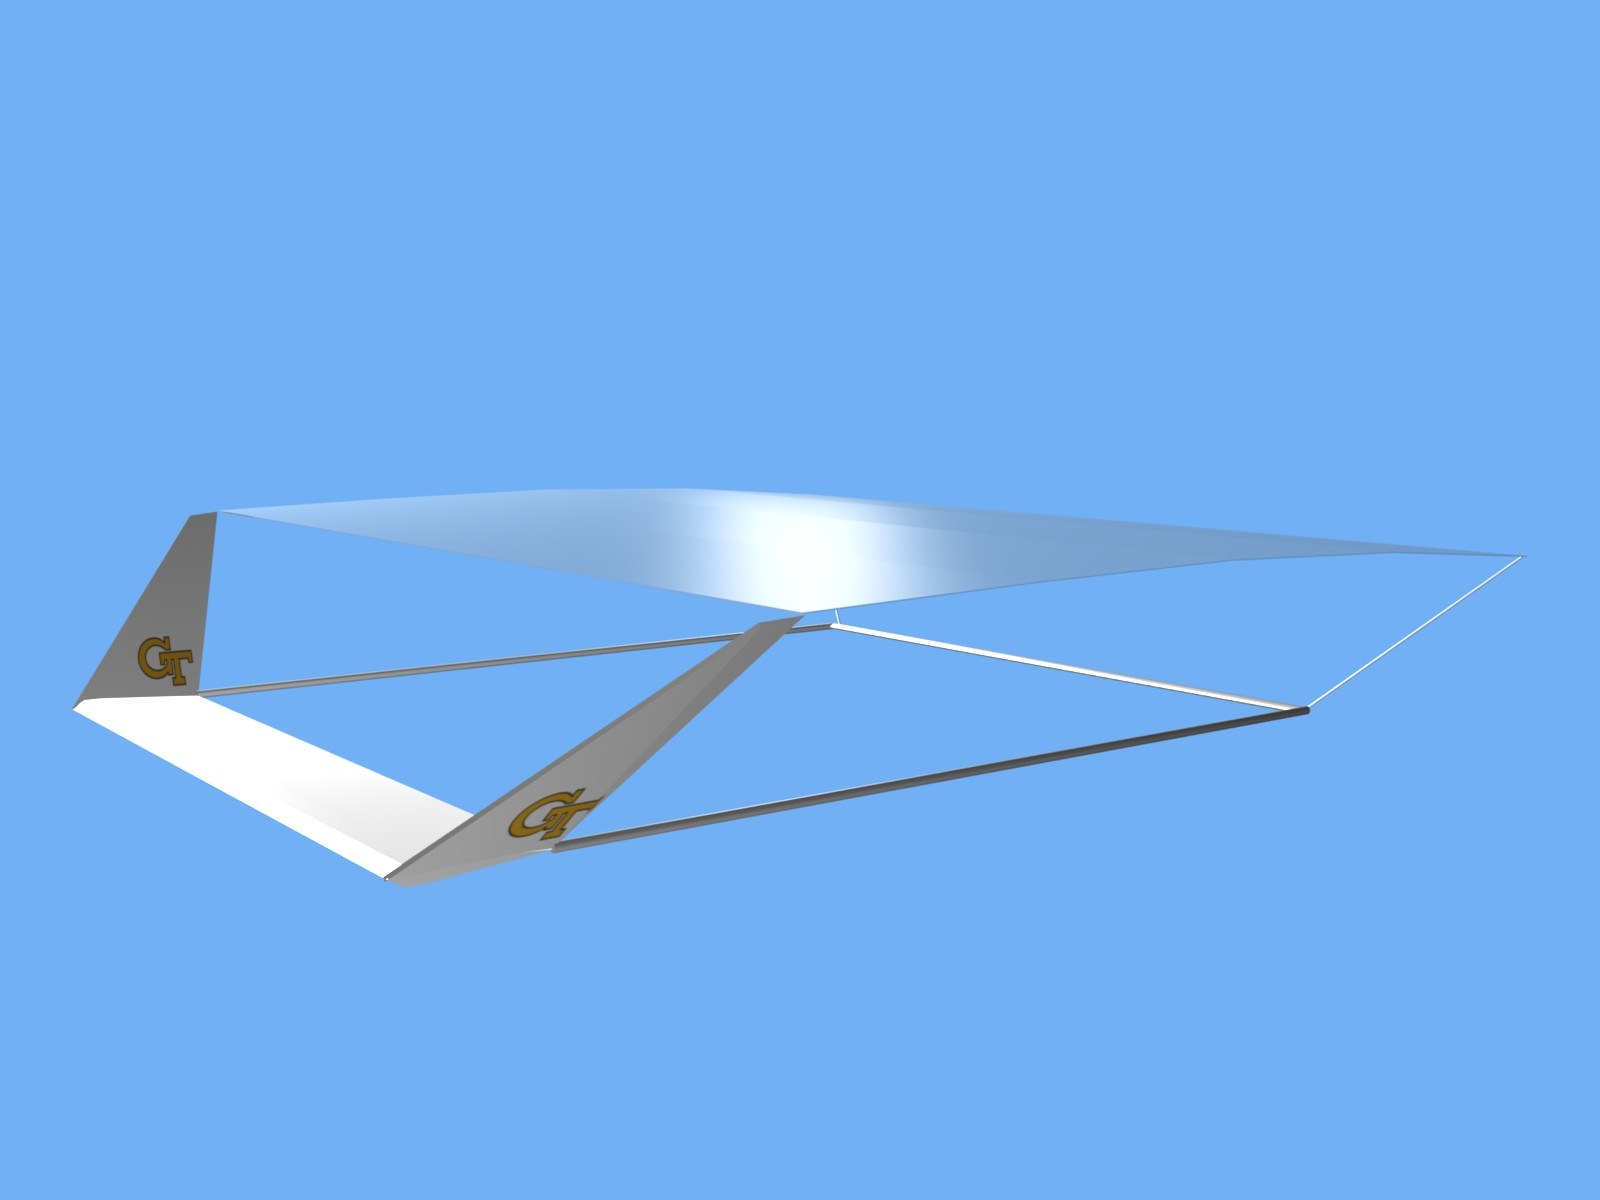
\includegraphics[width = 10cm]{FlyingCarpet.jpg}
\caption{An artist's concept of the Flying Carpet}
\end{figure}

This semester, the project focuses primarily on finding a suitable design for the reflector sheet on the Flying Carpet.
In particular, the sheet must
be prevented from oscillating or vibrating in a manner that will cause drag or structural failure, and it must be made to produce an
acceptable lift-to-drag ratio. The project aims to use wind tunnel experiments to discover which designs will work.

\chapter{Define Objectives}
In order of importance:

\begin{enumerate}

\item Discover what is necessary to obtain a lift-to-drag ratio which will allow the Flying Carpet to meet the mission requirements

\item Reduce flutter even further than in \cite{us}.

\end{enumerate}

\chapter{Prior Work}
During Spring 2018, flutter of a mylar sheet was investigated and several methods of reducing flutter were found. However,
flutter was not eliminated entirely, and the lift-to-drag ratio was far too low. \cite{us} Therefore, this semester the project will
focus on improving the lift-to-drag ratio. While testing the sheet, we will utilize the flutter-reduction techniques discussed in
\cite{us}, which are as follows:

\begin{enumerate}

\item Produce the sheet with concavely curved edges and attach elastic material under tension to its corners

\item Produce the sheet with concavely parabolic edges and attach a thread under tension to its leading and trailing
edges by means of smaller transverse threads

\item Use adhesive to attach the sheet strongly to the support structure along it's lateral edges with negligible room
to move
 
\end{enumerate}

We may modify these methods or devise new ones if it becomes apparent that they are reducing the lift-to-drag ratio.

\chapter{Project Schedule}

\begin{tabular}{|l|p{10cm}|p{10cm}|}
\hline
Date & Planned & Accomplished \\ \hline
21-08-2018 & Find out where experiments should be performed & Learned that the wind tunnel in MK104 is to be
used and obtained access to the schedule on T-Square \\ \hline
22-08-2018 & Take measurements of the sting balance for mounting models and obtain baseline lift and drag measurements & 
Discovered that the sting balance was missing and that we could alternatively construct our own force balance \\ \hline
23-08-2018 & Locate the sting balance & Discovered that the balance was under repair in the hands of the manufacturer (Aerolab) and
that it is not expected to be returned until the end of September \\ \hline
24-08-2018 & Construct a working setup to measure the drag produced by the model & Assembled the electronics necessary to read a
voltage from a load cell and proposed ideas for a mount which would transfer either drag or axial force to it \\ \hline
27-08-2018 & Evaluate different proposed mount designs and if necessary order materials & Redesigned mount based on advice from Prof. K. \\ \hline
28-08-2018 - 31-08-2018 & Construct the mount & Obtained and fabricated all subcomponents \\ \hline
03-09-2018 - 06-08-2018 & Finish constructing and testing the mount & Finished constructing the mount and passed basic tests \\ \hline
07-09-2018 & Introduce new members to their tasks & prepared the three members who appeared to begin work \\ \hline
10-09-2018 & Meet remaining members and ascertain when they are available & NA \\ \hline
11-09-2018 & Finish preparing the established mount & NA \\ \hline

\end{tabular}

\chapter{Experimental Setup}

\section{Model Details}
\section{Load Cell Details}
\subsection{Load Balance}
The experimntal setup from Spring 2018 cannot be reused because the force balance is under repair away from Georgia Tech. Therefore, an alternative
force balance system must be developed. Another force balance exists, but we doubt the accuracy of its drag measurements based on previous experience. So, to measure drag, we have constructed an axial force balance. The axial force balance uses a mechanical structure involving ball bearings
to transfer load in only one direction. The affects of moments, other components of force, and friction are minimal. It uses a 100g load cell
to measure force. The model will be attached to the axial force balance, and will rotate together with it as the angle of attack is changed.
The lift will be measured by the existing force balance, and when combined with the axial force measurements from the axial force balance,
the drag can be calculated.

There is some concern that the drag force on the axial force balance itself will interfere with measurements of the model's drag. In order to
take the drag of the balance into acount, tests will be performed on the balance without a model on it. The drag measured in these baseline tests
will be subtracted from the drag measured in model experiments. However, if the drag on the axial force balance is too high, then it may be difficult
to resolve the drag of the model. For that reason, the axial force balance was designed to be as small as possible in order to minimize its drag.

\section{Prediction of Expected Forces and Moments}

\subsection{From Boundary Layer Equations}
The drag on the sheet was predicted using a standard, well tested technique based on Blasius' equation. This technique assumes laminar flow,
the accuracy of which in our wind tunnel experiments is uncertain. Based on these assumptions, the following equation from \cite{Anderson} gives
the drag on each side of the sheet.
\[ C_f = \frac{1.328}{\sqrt{Re_c}} \]
Where $C_f$ is the drag coefficient and $Re_c$ is the chord-based Reynolds number. For a $60cm \times 30cm$ sheet at $9.8m/s$ in the wind
tunnel, this predicts a drag of $0.063N$.

\subsection{From CFD}
CFD in ANSYS Fluent was used to predict the lift and drag at nonzero angle of attack. A 2D, laminar, transient simulation was performed.
Since it is impractical to attempt to create a mesh fine enough to resolve the thickness of the sheet, a needle-like shape with sharp
leading and trailing edges was used. The maximum thickness was 1% of the chord. However, in hindsight, this is too thick, and another
simulation ought to be done with a thinner sheet. In any case, it should accurately capture the phenomena at the leading and trailing edge,
although it may overpredict the drag by a small amount.

At zero angle of attack, the drag predictions match that described in the previous section with $3\%$ error. However,
at nonzero angle of attack,
the drag is remarkable high. Also, the drag polar (Fig. \ref{cfd_polar}) does
not have the shape which is expected for airfoils. In order to investigate
the cause of the drag, a the magnitude of the flow velocity near the leading edge was rendered (Fig. \ref{flat_velocity}). There appears
to be a
standing vortex near the leading edge on the downwind side of the sheet. This is probably related to the phenomenon known as "vortex lift"
which occurs for wings with sharp leading edges.

It may be possible to avoid the vortex which is causing extra drag. Another simulation was done using a cambered sheet. The camber line
is an arc which subtends a $10\degree$ angle. This significantly improved the lift-to-drag ratio (Fig. \ref{cfd_polar}), since the sheet was
able to avoid the
leading edge vortex while simultaneously generating lift (Fig. \ref{cambered_velocity}). The lift-to-drag ratio is still not very impressive,
but this can probably be
improved by designing the camber line less naively.

\begin{figure}
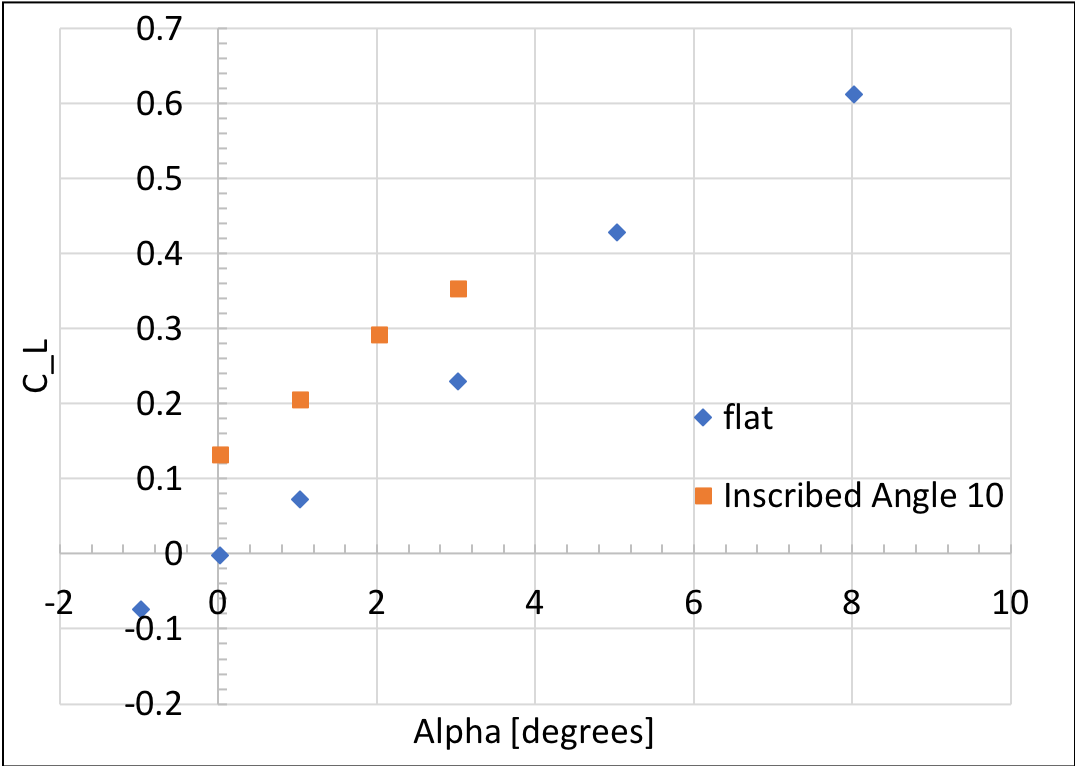
\includegraphics[width = 10cm]{lift.png}
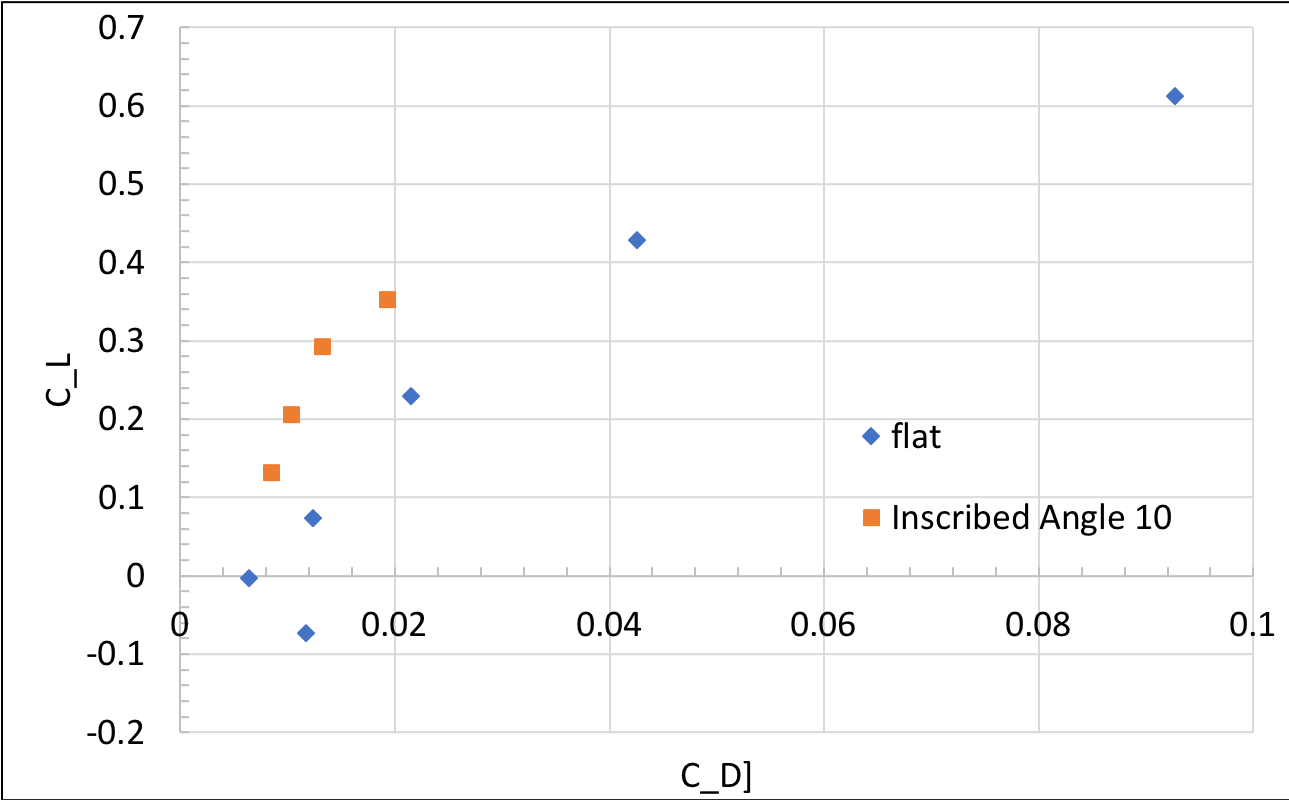
\includegraphics[width = 10cm]{polar.png}
\caption{Lift and drag data from CFD simulations of both sheets}
\label{cfd_polar}
\end{figure}

\begin{figure}
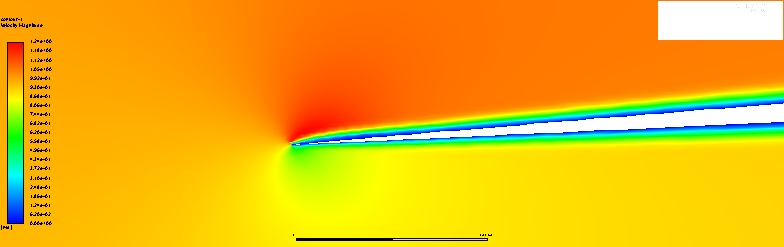
\includegraphics[width = 20cm]{alpha2.jpg}
\caption{The cambered sheet at $\alpha = 2\degree$}
\label{cambered_velocity}
\end{figure}

\begin{figure}
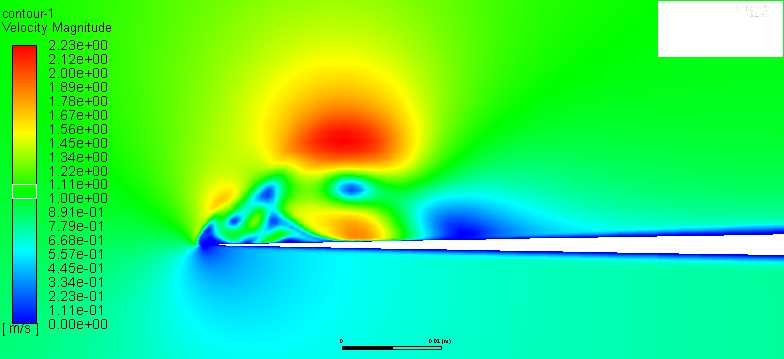
\includegraphics[width = 20cm]{flat.jpg}
\caption{The flat sheet at $\alpha = 5\degree$}
\label{flat_velocity}
\end{figure}

\begin{thebibliography}{3}

\bibitem{us}
Micaiah C. Smith-Pierce, Yana Charoenboonvivat, Dhwanil Shukla, and Narayanan M. Komerath. ``High Altitude Aerodynamic Reflectors To
Counter Climate Change'', 2018 Applied Aerodynamics Conference, AIAA AVIATION Forum, (AIAA 2018-3963)
\verb|https://doi.org/10.2514/6.2018-3962|

\bibitem{Anderson}
John Anderson, \textit{Fundamentals of Aerodynamics}, 6th edition

\end{thebibliography}

\end{document}
